%=============================================================================
% Thesis Template in LaTex
%
% File:  07-Schlussfolgerung.tex -- Schlussfolgerung und Ausblick
% Author(s): Cyrano Golliez <golliezc@student.ethz.ch>
%
% Creation:  27 Jan 2014
% Time-stamp: <Tue 2013-08-13 20:14 juergen>
%
% Copyright (c) 2014 Infrastructure Management Group (IMG)
%               http://ibi.ethz.ch
%
% More information on LaTeX: http://www.latex-project.org/
%=============================================================================

\chapter{Schlussfolgerung und Ausblick}
\label{chap:Schlussfolgerung}


Basierend auf den in Abschnitt \ref{chap:Resultate} dargestellten Resultaten und der in Abschnitt \ref{chap:Diskussion} druchgeführten Diskussion der Resultate, ist die Variante 2 die optimale Verbesserung der Verkehrssituation in Uster. Unter den in Abschnitt \ref{sec:Kostenstruktur} getroffenen Annahmen und der unter Abschnitt \ref{subsec:Modellierung} modellierten Veränderungen des Mobilitätsbedarf, ergibt sich, dass sich die Mehrkosten die beim Bau der Variante 2 gegenüber dem Bau der Variante 1, bei einer Betrachtung der Gesamtkosten die von einer Variante über den Zeitraum von 40 Jahren generiert werden, lohnen würden. Insbesondere unter der in Abschnitt \ref{chap:Diskussion} durchgeführten, näheren Betrachtung der Reisezeitkosten, ergibt sich eine eindeutige Lösung, zur Optimierung des Bahnübergangss Brunnenstrasse. Somit ist die Variante 2 nicht nur in ökologischer Hinsicht der Variante 1 überlegen, sondern auch im ökonomischen Sinne, da sich die grösseren Investitionen, bei einer Betrachtung über einen Zeitraum von 40 Jahren, bei weitem lohnen würden. Hinzukommt, dass die geplante Velounterführung der Variante 2, eine Reduktion der Belastung der Öffentlichkeit, in Form der Reduktion der Schadstoffemission erreichen würde. 

Die höheren Investitions- und Wartungskosten der Variante 2 rechnen sich demnach im Vergleich zur Variante 1, bei einer Betrachtung der Situation über 40 Jahre. Die Variante 3, die weitaus höhere Investitionskosten verursachen würde, lohnt sich, nach der in Abschnitt \ref{chap:Resultate} und Abschnitt \ref{chap:Diskussion} durchgeführten Diskussion der Risiken, aufgrund der höheren Reisezeitkosten die infolge der verlängerten Wartezeit entstehen, nicht. \\
Ausser im vierten Zustand der Sensitivitätsanalyse, in der die zu erwartende Reisezeit verändert wird, kann die Variante 3, aufgrund der höheren Gesamtkosten, als optimale Variante ausgeschlossen werden. Somit lohnen sich die Mehrkostend der Variante 3 nicht.

Anzumerken ist, dass sich die Ergebnisse bei der Berücksichtung weiterer Interessengruppen sowie einer komplexere Modellierung der Einflussfakoten auf das DTV, verändern könnten.
Desweiteren wäre eine Betrachtung der Interessen und Kosten des öffentlichen Nahverkehrs in Uster, um die Verkehslage am Bahnübergang möglichst realitätsgetreue abzubilden, unerlässlich. Ausserdem wären die Auswirkungen die vom Bau einer Variante auf die Anwohner sowie auf die Umwelt ausgehen würden, ein weiterer wichtiger Aspekte der im Entscheidungsprozess berücksichtigt werden müsste.  \\
Aufgrund der begrenzten Möglichkeiten die mir im Rahmen dieser Projektarbeit zur Beurteilung der Situation zur Verfügung standen, konnte ich nicht alle relevanten Faktoren in der Entscheidungsfindung berücksichtigen, was im Rahmen einer erweiterten Studie zur Situation am Bahnübergang Brunnenstrasse erfolgen sollte.

Zu Beginn des von mir durchgeführten Problemlösungsprozesses, habe ich zur Vereinfachung die beteiligten Personen, auf die in Abschnitt \ref{subsec:Gruppen} defnierten Interessensgruppen reduziert, um im gegeben Zeitrahmen eine ansprechende Lösung erarbeiten zu können. 
Eine Aufteilung der Kosten nach den verschiedenen Interessensverbänden wäre im Rahmen der Diskussion sehr aufschlussreich gewesen. Da die die Situation und die Möglichkeiten die mir für die Modellierung zur Verfügung standen zur Folge haben, dass die Reisezeitkosten den gesamten Risikovergleich der Varianten bestimmten, habe ich im Rahmen der Diskussion der Ergebnisse auf diese Unterteilung verzichtet. Es wäre jedoch sehr interessant, im Rahmen der weiteren Prüfung der Varianten, eine vertieftere Beurteilung der Nutzer- und Besitzerkosten durchzuführen.

Hinsichtlich der zukünftigen Entwicklung der Mobilität wird das Fahrrad vorraussichtlich auch auf Strecken bis zu 30km eine entscheidende Rolle bei der Verkehrsmittelwahl spielen. Aufgrund dessen und in anbetracht der Bestrebungen der Stadt Uster ein Zentrum von regionaler Bedeutung zu werden, ist die Förderung des ökologischen und zukunftsorientierten Langsamverkehrs unerlässlich und insbesondere im Rahmen einer nachhaltigen Stadtentwicklung voranzutreiben. \\
So wäre eine Erweiterung der geplanten Veloinfrastruktur entlang der Pfäffikerstrasse bis zum Spital sowie entlang der Bahnhofstrasse bis zum Sternenplatz, im Rahmen einer vertiefen Untersuchung zu berücksichtigen. Eine mögliche Variante einer solchen Veloschnellroute könnte, anhand des Beispiels der Radschnellwege von Kopenhagen erstellt werden. Ein solches Beispiel, wäre die C99 in Kopenhagen-Albertslund. Diese sogenannte \textit{Super-Radschnellrouten} auch bekannt als \textit{Cykelsuperstier} haben sich in Dänemark bereits bewährt und haben das Pendeln mit dem Velo, leichter und sicherer gemacht.  
Insbesondere unter Anbetracht der akutellen Situation mit CoVid-19, in der das Velo eine Renaissance erlebt, muss der Ausbau und die Förderung der innerstädtischen Langsamverkehrsnetze voran getrieben werden.

Nichtsdestotrotz ist, um eine nachhaltige Verbesserung der Verkehrslage in Uster zu erreichen, eine Berücksichtung der weiteren Schwachstellen des Ustemer Verkehrsnetz unerlässlich. Inbesondere die zukünftige Entwicklung des Nüsslikreisel sowie der Zürichstrasse haben einen grossen Einfluss auf die Stadtentwicklung. Hinzukommt, dass die Optimierung eines Teilstücks einer bestehenden Infrastruktur nur dann erfolgen sollte, wenn die Einflüsse auf die umliegenden Systeme berücksichtigt werden. So muss um Uster nachhaltig zu verbessern, nicht nur das Velonetz ausgebaut sondern das gesamte Verkehrskonzept der Stadt überarbeitet werden. 

Die von mir vorgeschlagenen Schritte die Uster in der nächsten Zeit tätigen soll oder kann sind in der nachfolgenden Abbildung \ref{img:UsterFuture} dargestellt. \\
So ergibt sich einerseits, wie ausführlich besprochen, der Weg die Variante 2 in Betracht zu ziehen und die weitere Schritte dementsprechend einzuleiten, wie zum Beispiel der Beginn einer Detailstudie oder aber bereits der Start des Planungsprozesses. Der zweite Weg der sich der Stadt Uster bietet, ist eine weitere Hauptstudie, wodurch infolge der ausführlichen Prüfung der Situation, entweder die Wahl der optimalen Variante manifestiert oder aber eine andere Variante als die als optimal zu erachtende Variante bestimmt wird. Die letzte Möglichkeit die sich der Stadt Uster bietet, ist die Option: Variante 1 - "nichts zu machen", wobei für relativ wenig Geld die Verkehrssicherheit marginal erhöht wird. 

\begin{figure}[h!]
	\centering
	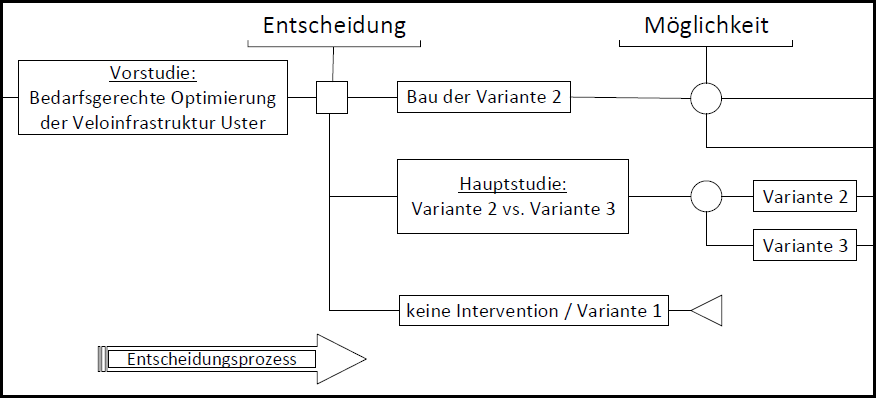
\includegraphics[width=.6\textwidth]{figures/f-07-01-EntscheidungsprozessUster}
	\caption[Entscheidungsprozess der Stadt Uster]{Möglicher Entscheidungsprozess der Stadt Uster für die nähere Zukunft}
	\label{img:UsterFuture}
\end{figure} 

\pagebreak

\paragraph{Ausblick}

Das betrachtete Problemfeld der im Rahmen dieser Projektarbeit gestellten Aufgabenstellung ist sehr umfangreich. Um ein ansprechendes Resultat im gegebenen Zeitrahmen erarbeiten zu können, mussten einige Vereinfachungen und Annahmen gemacht und ein Schwerpunkt auf ein System gelegt werden. Es hätten demnach einige weiter Punkte berücksichtigt sowie gewisse Akspekte genauer modelliert werden können. \\
So hätten zum einen die Interessensgruppe der Nutzer differenzierter betrachtet und um die Fussgänger erweitert werden können. Im gleichen Zuge hätte der Öffentliche Verkehr in die Entscheidungsfindung miteinbezogen werden müssen, was in Anbetracht dessen, dass der Bahnübergang Brunnenstrasse im Busnezt ein zentraler Knotenpunkt ist, in einer vollumfänglichen Betrachtung der Situation unerlässich ist. Zusätzlich hätten politische Entscheidungen sowie Budgetgrenzen der Stadt Uster und des Kantons Zürich berücksichtigt werden können, um eine politisch tragbare und realitätsnahe optimale Variante erarbeiten zu können.

Um eine genauere Vorhersage der Zukunft von Uster machen zu können, wäre das Berücksichtigen weiterer Szenarien und demnach weitere Einflussfaktoren notwendig. Durch die Berücksichtigung weiterer Einflussfaktoren wird die Modellierung der Parameter sowie die Risikoberechnung der Varianten komplizierter jedoch das Resultat der Optimierung exakter. 
So wäre eine Verkehrssimulation, mit der die effektive Verkehrslage in der Stadt modelliert wird, ein geeignetes Mittel, um zum Beispiel im Falle der Variante 3 die entstehende Wartezeit aufgrund des Ampelsystems genauer zu bestimmen. Mithilfe von Verkehrssimulation wäre demnach ein exakteres Resultat zu erwarten und die Infrastruktur der Varianten könnte auf ihre Gebrauchstauglichkeit untersucht werden. Zusättzlich wäre das Modellieren der Verkehrssicherheit der verschiedenen Varianten ein wichtiger Schritt, um die effektive Gefahrenlage, die von einer jeweiligen Variante ausgeht, in die Wahl der optimalen Variante miteinzubeziehen.\\
Und abschliessend wäre 
  



% ===========================================================================
% EOF
%

%%% Local Variables:
%%% mode: latex
%%% TeX-master: "../main"
%%% End:
